%Lo hecho con imagenes es temporal, tal vez provisiempre
\part*{Ejercicio 7}
%Se nos solicitó implementar mediante compuertas lógicas un contador asincrónico y otro sincrónico, ambos %de 3 bits y determinar la máxima velocidad de opeación de ambos.

\subsection*{Contador Asincrónico}
Para el contador asincrónico se siguió el esquema mostrado en la Figura \ref{7_fig1}. Se implementó utilizando Flip-Flops JK mediante integrados 74HC112, como puede observarse en la Figura \ref{7_fig2}. Utilizamos una señal cuadrada otorgada por el generador de señales, de 5V con un ciclo de trabajo del 50\%. En particular nuestro contador va de 7 a 0, cuenta hacia atrás, trabaja con flancos descendentes del Clock para el bit menos significativo y con flancos ascendentes para los últimos 2 bits.

%\begin{figure}[H]
%\begin{center}
%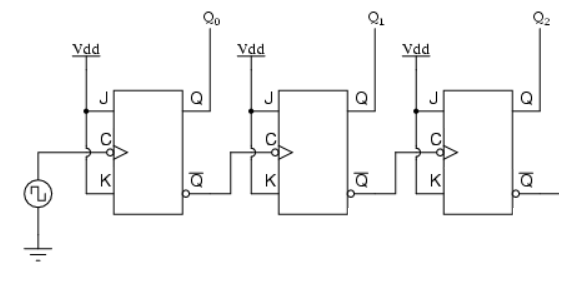
\includegraphics[scale=0.25]{ejercicio7/imagenes/asynccircuito.png}
%\caption{Circuito utilizado para el contador asincronico} \label{7_fig1}
%\end{center}
%\end{figure}

\begin{figure}[H]
\begin{center}
  \begin{minipage}[b]{0.4\textwidth}
  	\begin{center}
  		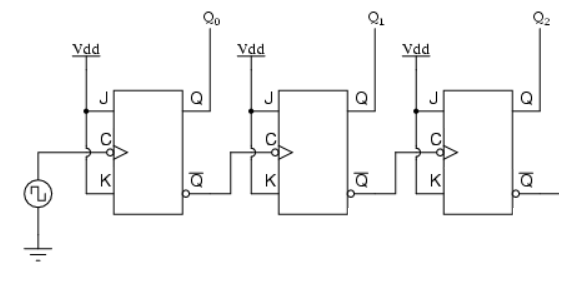
\includegraphics[scale=0.25]{ejercicio7/imagenes/asynccircuito.png}
  	\end{center}
  \caption{Circuito utilizado}
  \label{7_fig1}
  \end{minipage}
  \begin{minipage}[b]{0.4\textwidth}
    \begin{center}
  		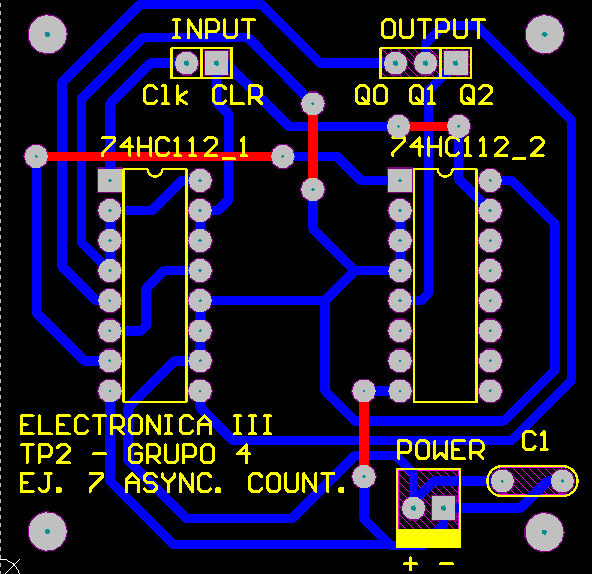
\includegraphics[scale=0.25]{ejercicio7/imagenes/asyncaltium.png}
	\end{center}
  \caption{Implementación con 74HC112}
  \label{7_fig2}
 \end{minipage}
\end{center}
\end{figure}


%Los flip-flops se conectan en cascada, donde se utiliza la salida $Q$ o $Q^{*}$ (dependiendo si queremos trabajar con flancos ascendentes o descendentes) conectada a la entrada clock de cada flip-flop después del primero. Al primero se conecta la señal deseada como Clock, nosotros utilizamos una señal cuadrada otorgada por el generador de señales, de 5V con un ciclo de trabajo del 50\%. En particular nuestro contador va de 7 a 0, cuenta hacia atrás, trabaja con flancos descendentes del Clock (cuando este pasa de valer 1 a 0) para el bit menos significativo y con flancos ascendentes para los últimos 2 bits( cuando el bit anterior pasa de 0 a 1) ya que los integrados 74HC112 tienen la entrada del clock negada y le conectamos $Q^{*}$, lo que equivale a conectar $Q$. Esto puede observarse junto a su correcto funcionamiento en la Figura \ref{7_fig3} donde si vamos desde arriba hacia abajo tenemos el Clock, $Q_0$ (bit menos significativo) ,$Q_1$ y $Q_2$.


%\begin{figure}[H]
%\begin{center}
%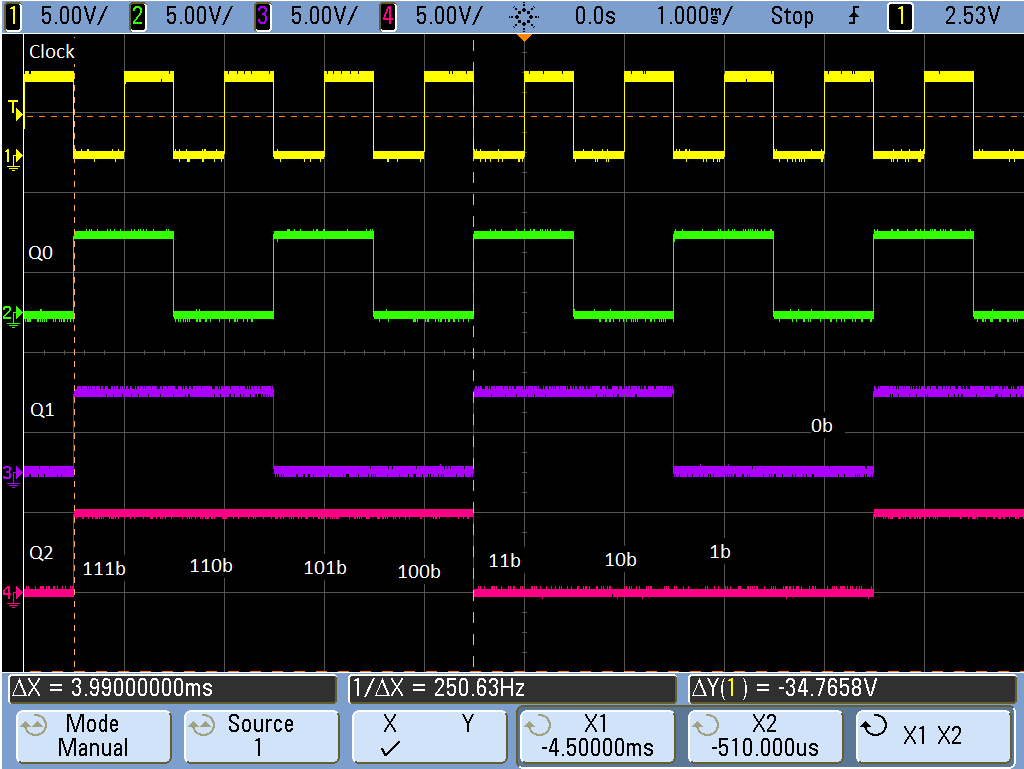
\includegraphics[scale=0.25,left]{ejercicio7/imagenes/async.png}
%\caption{Comportamiento del contador} \label{7_fig3}
%\end{center}
%\end{figure}

%\begin{wrapfigure}{l}{6.5cm}
%\begin{center}
%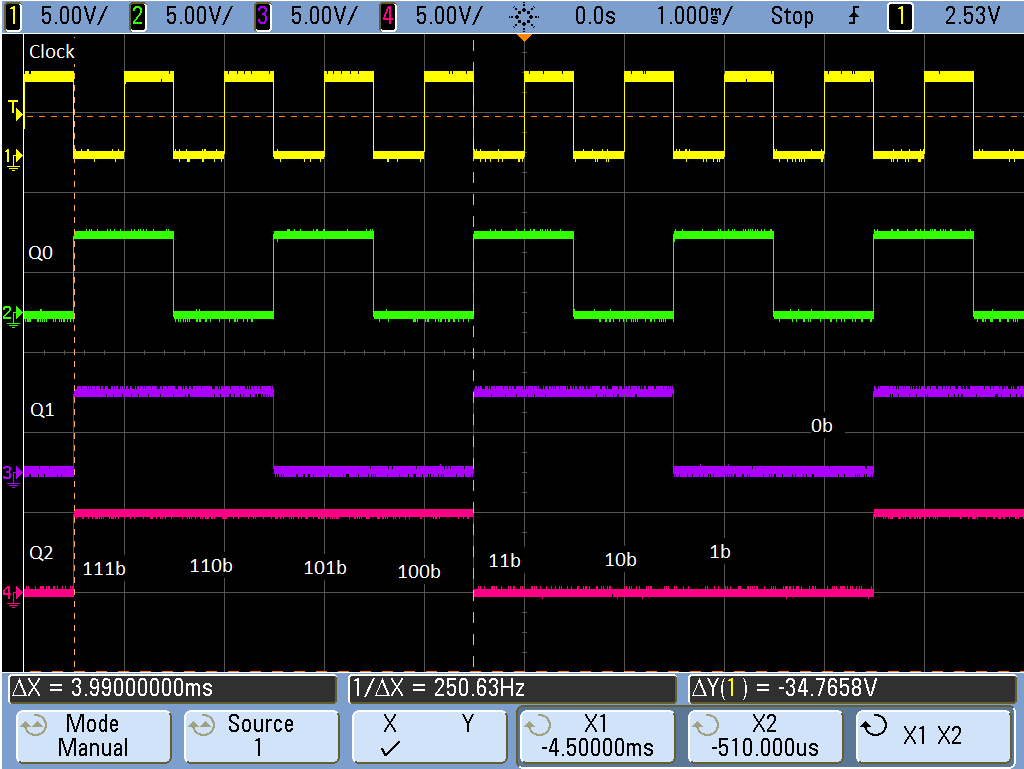
\includegraphics[scale=0.25,left]{ejercicio7/imagenes/async.png}
%\caption{Comportamiento del contador}\label{7_fig3}
%\end{center}
%\end{wrapfigure} 

%A modo de aclaración, podemos notar también en la Figura \ref{7_fig3} que mientras el bit menos significativo cambia con el flanco descendente del Clock, cuando este pasa de valer 1 a 0, los otros bits cambian cuando el bit anterior pasa de valer 0 a 1 ya que en nuestro caso la señal que le llega a cada entrada clock de los últimos dos flip-flops se encuentra conectada $Q^{*}$ pero las entradas clock de los integrados 74HC112 estan negadas, por lo que equivaldría a enviar la señal $Q$.

%En este tipo de contador, las salidas (que representan a los bits) no cambian exactamente al mismo
%En este tipo de contador 

\begin{wrapfigure}{l}{6.5cm}
\begin{center}
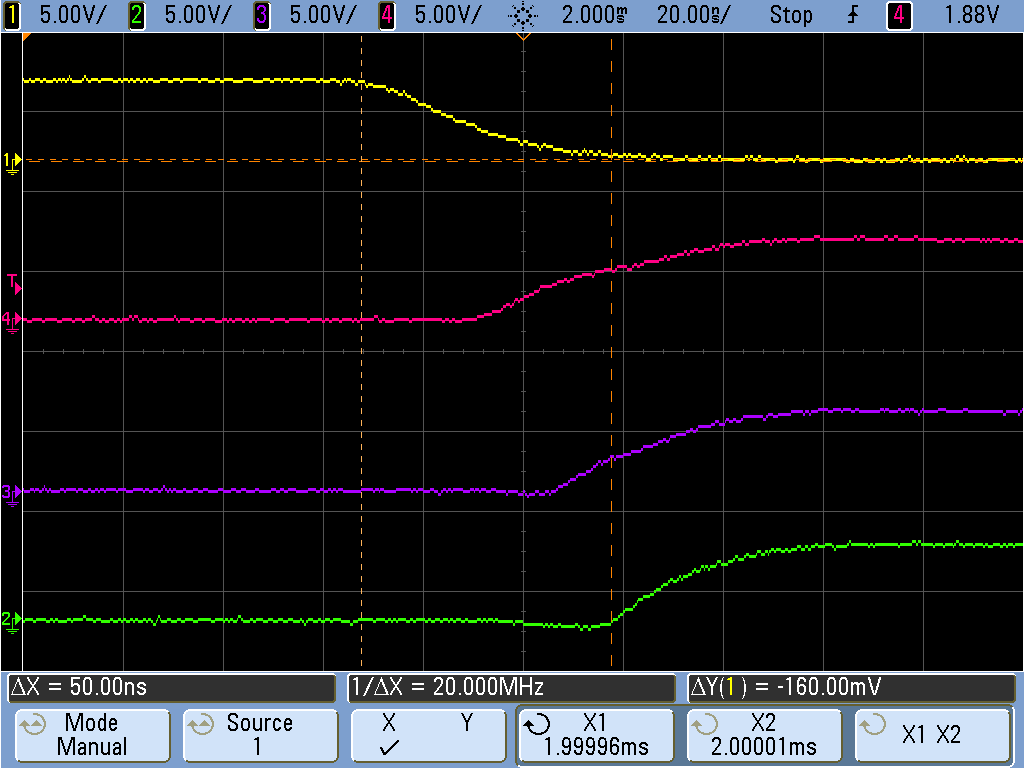
\includegraphics[scale=0.25]{ejercicio7/imagenes/timepropagation.png}
\caption{Medicion del delay acumulado}\label{7_fig3}
\end{center}
\end{wrapfigure}

Las salidas no cambian al mismo tiempo, hay un delay entre que la señal conectada a la entrada clock del flip-flop cambia hasta que la salida correspondiente también lo hace, entonces tenemos un delay total más grande a mayor cantidad de flip-flops conectados en cascada, habrá un mayor retraso entre que la señal del clock cambia y lo hace el bit más significativo. Esto es una desventaja de estos contadores porque hay que tener cuidado con la velocidad con la que trabaja el circuito ya que esta no puede superar la frecuencia que se obtiene luego de medir el máximo delay acumulado por todas las compuertas, también sucede con estos contadores que pasamos por estados falsos hasta llegar a cambiar el bit más significativo pero cambia tan rápido que esto no suele ser un problema grave para muchas aplicaciones.

Medimos el tiempo de propagación total desde que la señal del Clock comienza a descender hasta que el bit más significativo ($Q_2$) comienza a elevarse y obtuvimos un valor de 50 ns (ver Figura \ref{7_fig3}), observamos el datasheet y el fabricante nos dice que trabajando a 5V y a 25 ºC el tiempo de propagación de cada flip-flop es de 17 ns, con las 3 compuertas tendríamos 51 ns por lo que comprobamos que lo medido es aproximado al valor teórico esperado. En las Figuras \ref{7_fig4},\ref{7_fig5},\ref{7_fig6},\ref{7_fig7} podemos ver el comportamiento del circuito a medida que aumentamos la frecuencia del Clock, a grandes frecuencias podemos ver como las señales medidas empiezan a tener un comportamiento extraño que puede deberse a que el ancho de banda del osciloscopio que utilizamos no era el suficiente y que este esta interviniendo en las mediciones, pero a grandes rasgos podemos notar que a pesar de todo se mantiene entre los valores que el integrado detecta como 1 y como 0 según sea el caso, pero al llegar a 23.8 MHz podemos ver que los valores de las salidas tooglean, varían entre 0 y 1 y esto se debe a que ya mi tiempo de delay es mayor al periodo de la señal con la que estoy trabajando, al mirar el datasheet observamos que el fabricante nos dice que en las condiciones que trabajamos no debemos de pasar los 70 MHz, y esto dividido entre los 3 flip-flops me da 23.33 MHz.

%esto acarrea otro problema el cual es que de esta manera no puedo pasar directamente de un número a otro, dependiendo el caso paso por más o menos estados falsos. Esto no es un problema para la mayoría de los casos ya que los cambios son muy rápidos, por lo que es tolerable para distintas aplicaciones.

%\begin{figure}[H]
%\begin{center}
%  \begin{minipage}[b]{0.4\textwidth}
%  	\begin{center}
%  		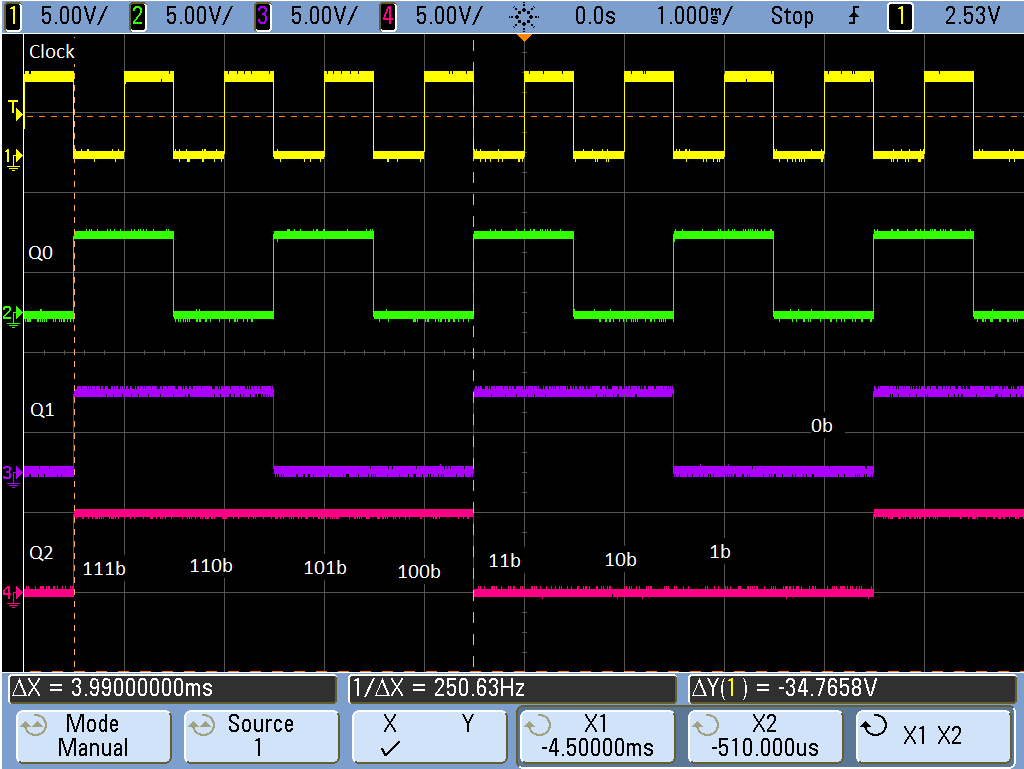
\includegraphics[scale=0.25]{ejercicio7/imagenes/async.png}
%  	\end{center}
%  \caption{Comportamiento del contador}
%  \label{7_fig3}
%  \end{minipage}
%  \begin{minipage}[b]{0.4\textwidth}
%    \begin{center}
%  		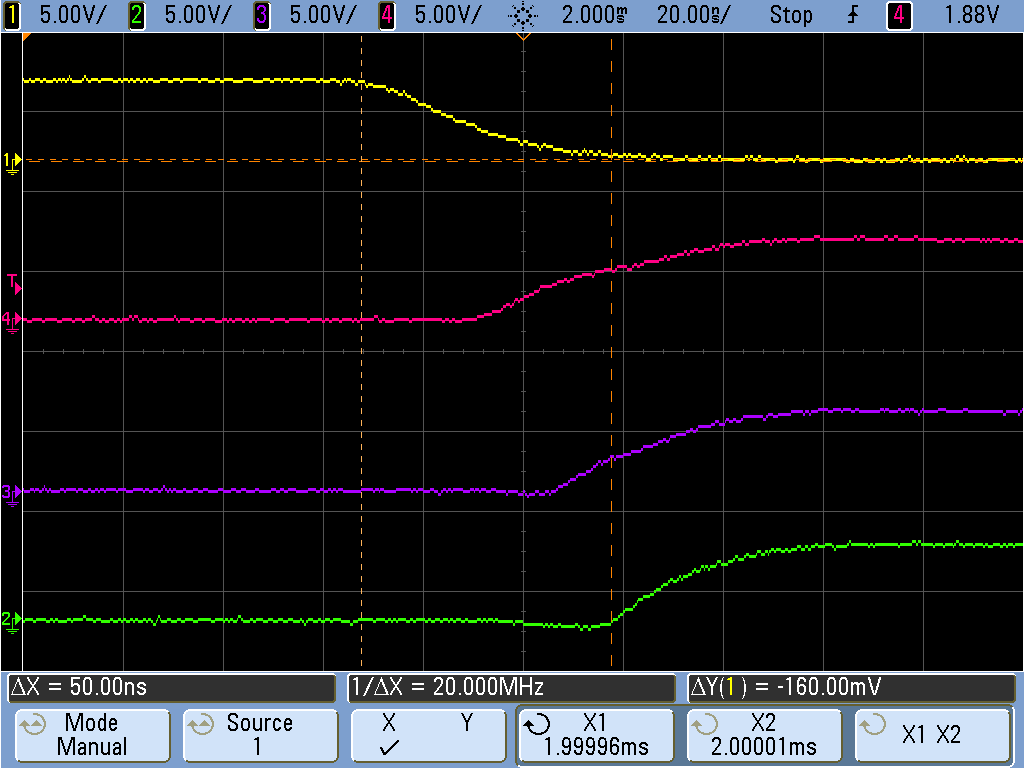
\includegraphics[scale=0.25]{ejercicio7/imagenes/timepropagation.png}
%	\end{center}
%  \caption{Medicion del delay acumulado}
%  \label{7_fig4}
% \end{minipage}
%\end{center}
%\end{figure}

\begin{figure}[H]
\begin{center}
  \begin{minipage}[b]{0.4\textwidth}
  	\begin{center}
  		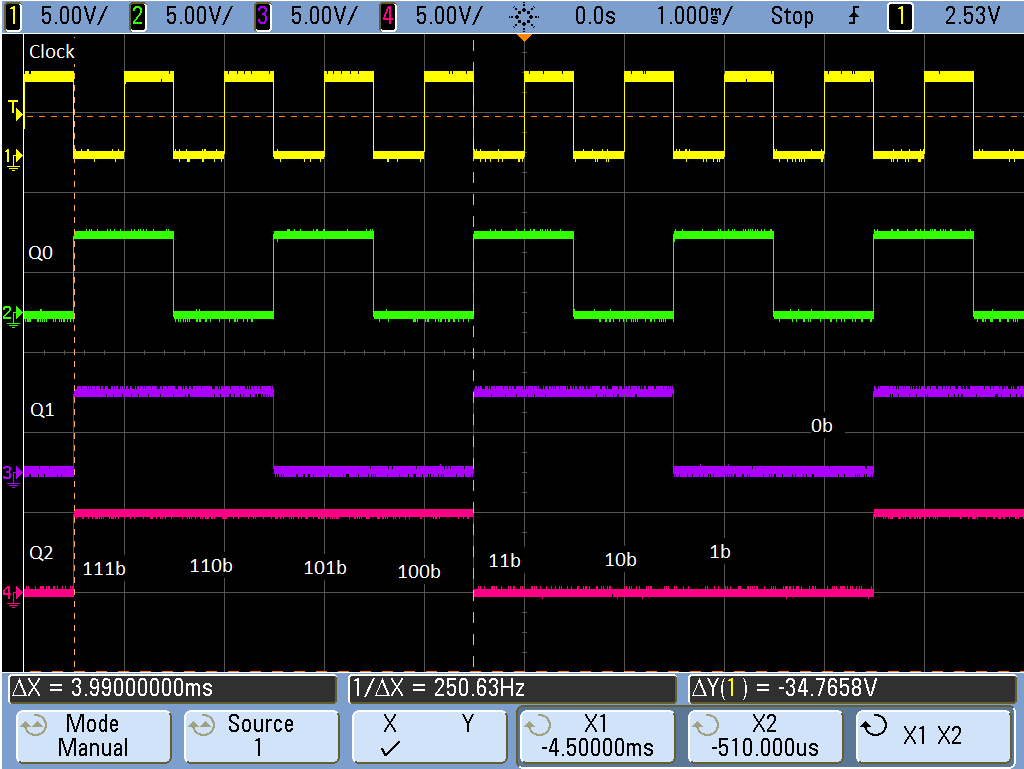
\includegraphics[scale=0.2]{ejercicio7/imagenes/async.png}
  	\end{center}
  \caption{Comportamiento a bajas frec}
  \label{7_fig4}
  \end{minipage}
  \begin{minipage}[b]{0.4\textwidth}
  	\begin{center}
  		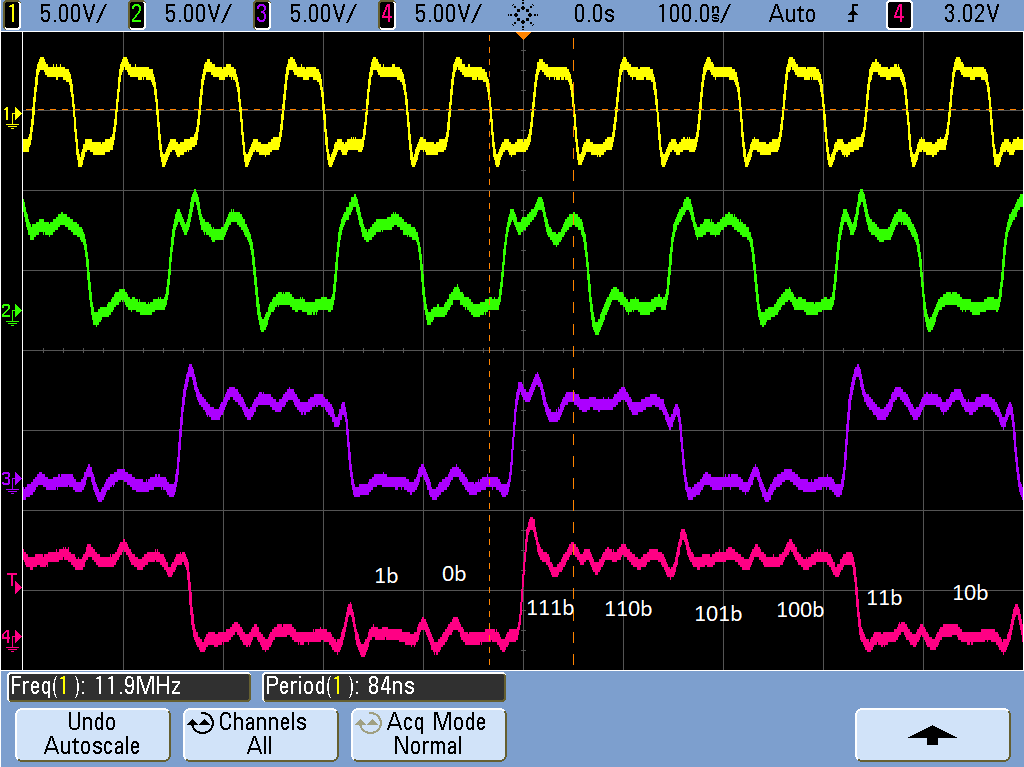
\includegraphics[scale=0.2]{ejercicio7/imagenes/async2.png}
  	\end{center}
  \caption{Comportamiento a 11.9 MHz}
  \label{7_fig5}
  \end{minipage}
  \begin{minipage}[b]{0.4\textwidth}
    \begin{center}
  		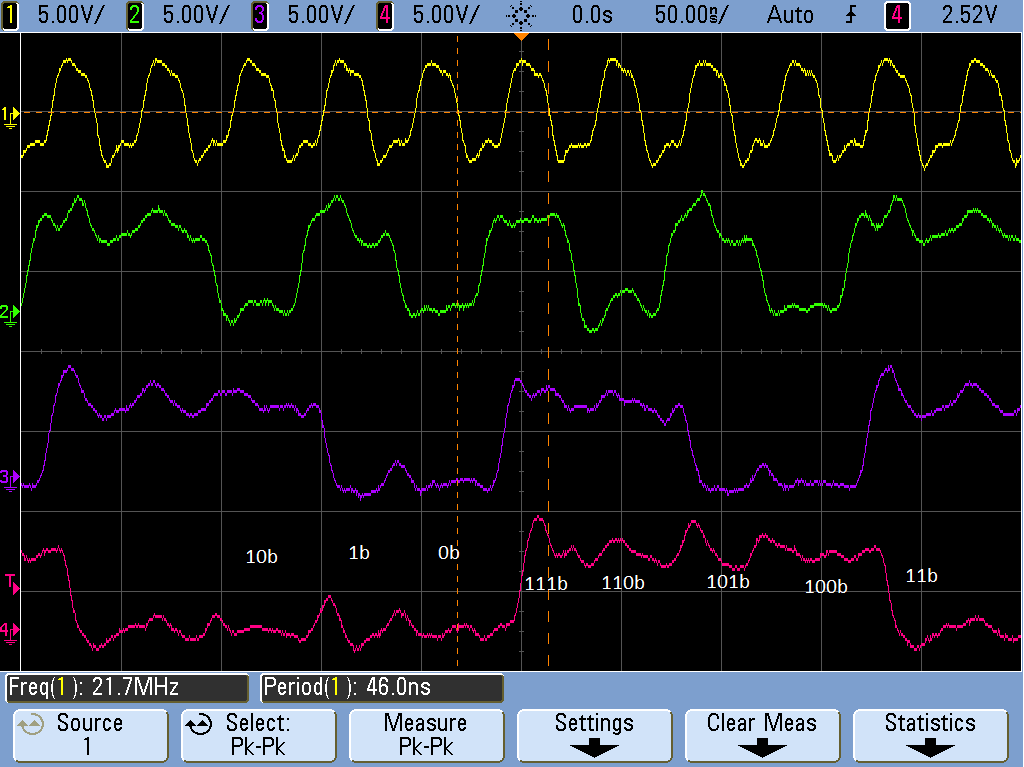
\includegraphics[scale=0.2]{ejercicio7/imagenes/async3.png}
	\end{center}
  \caption{A 21.7 MHz}
  \label{7_fig6}
 \end{minipage}
   \begin{minipage}[b]{0.4\textwidth}
    \begin{center}
  		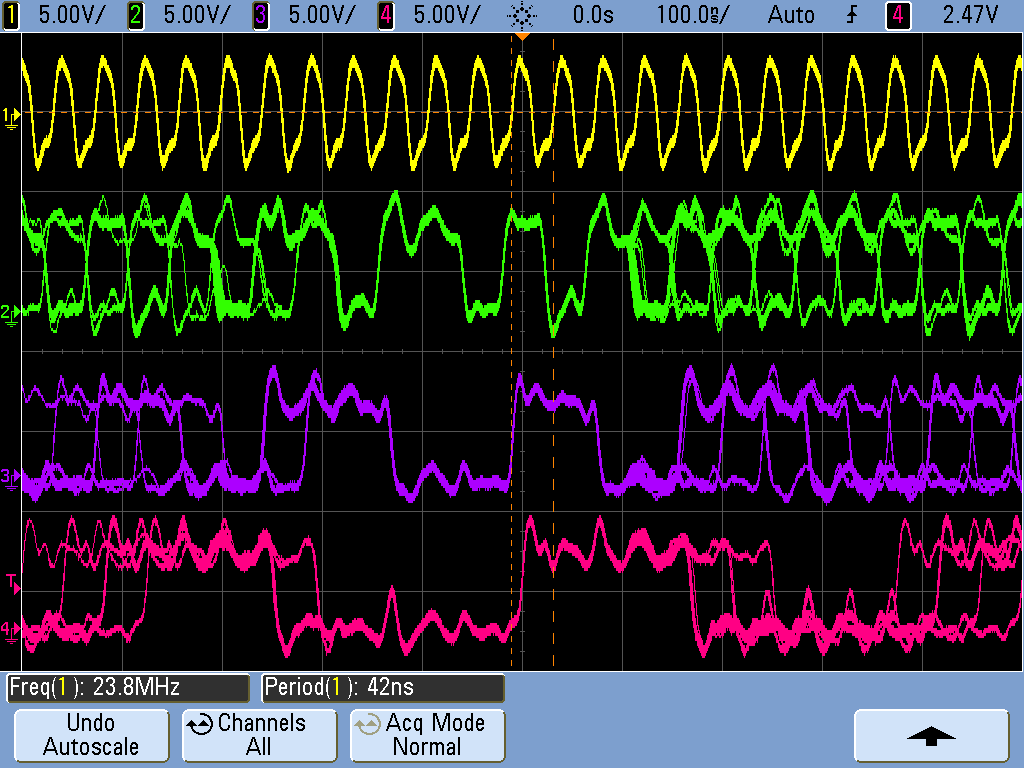
\includegraphics[scale=0.2]{ejercicio7/imagenes/async4.png}
	\end{center}
  \caption{A 23.8 MHz}
  \label{7_fig7}
 \end{minipage}
\end{center}
\end{figure}

%\begin{wrapfigure}{l}{6.5cm}
%\begin{center}
%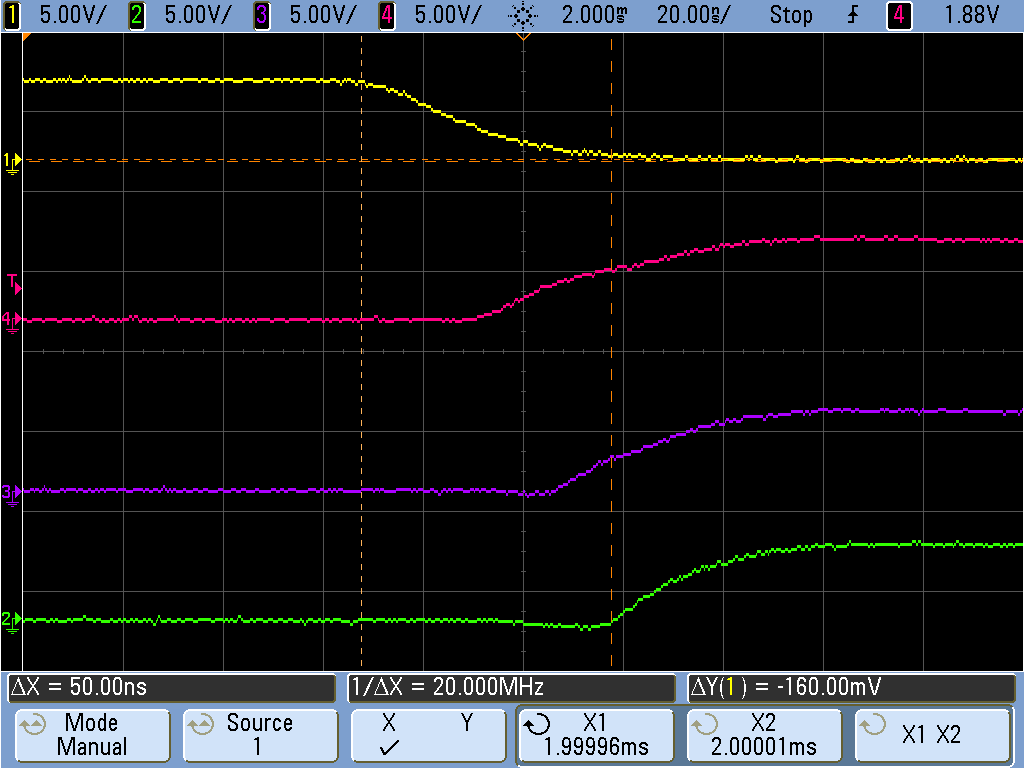
\includegraphics[scale=0.25,left]{ejercicio7/imagenes/timepropagation.png}
%\caption{Comportamiento del contador}\label{7_fig4}
%\end{center}
%\end{wrapfigure}
 


%\begin{figure}[H]
%\begin{center}
%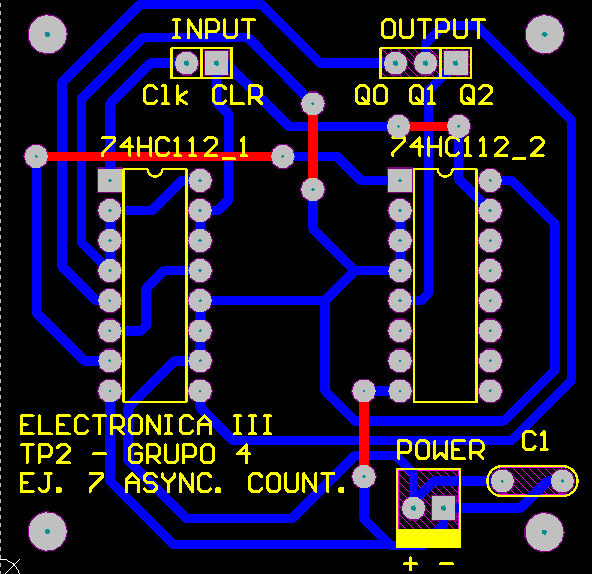
\includegraphics[scale=0.25]{ejercicio7/imagenes/asyncaltium.png}
%\caption{Implementación con 74HC112} \label{7_fig2}
%\end{center}
%\end{figure}

\subsection*{Contador Sincr\'onico}
Este contador que avanza de forma ascendente. La diferencia con el anterior es que los clock de cada Flip-Flop estar\'an conectados directamente a la misma señal en lugar de usar la señal del flip-flop anterior, se puede observar en la Figura \ref{7_fig8}. Este cambio har\'a que cada parte se active con el flanco descendente de la misma señal, reaccionando todas las partes del contador a un mismo tiempo determinado, siempre y cuando se trate del mismo componente o tengan las mismas caracter\'isticas temporales, y no obtener un arrastre en el delay final.
\newline
Al mirar el tiempo de propagaci\'on de este circuito (Figura \ref{7_fig9}) obtenemos que solo hay 24ns de delay, 17ns correspondiente al flip-flop (ahora no se suman sus delay porque son independientes) y 7ns correspondientes a la compuerta AND del circuito, esto quiere decir que reci\'en a los 42,66MHz el circuito empezar\'a a togglear porque el tiempo de delay superar\'a la frecuencia de trabajo al igual que en el caso anterior. No pudimos obtener im\'agenes de este caso porque se necesita tener un osciloscopio de m\'as de 200MHz debido a que si el instrumento no tiene un ancho de banda 5 veces mayor a la frecuencia de trabajo se perder\'an detalles de la señal que impiden tener una medici\'on correcta.

\begin{figure}[H]
\begin{center}
  \begin{minipage}[b]{0.4\textwidth}
  	\begin{center}
  		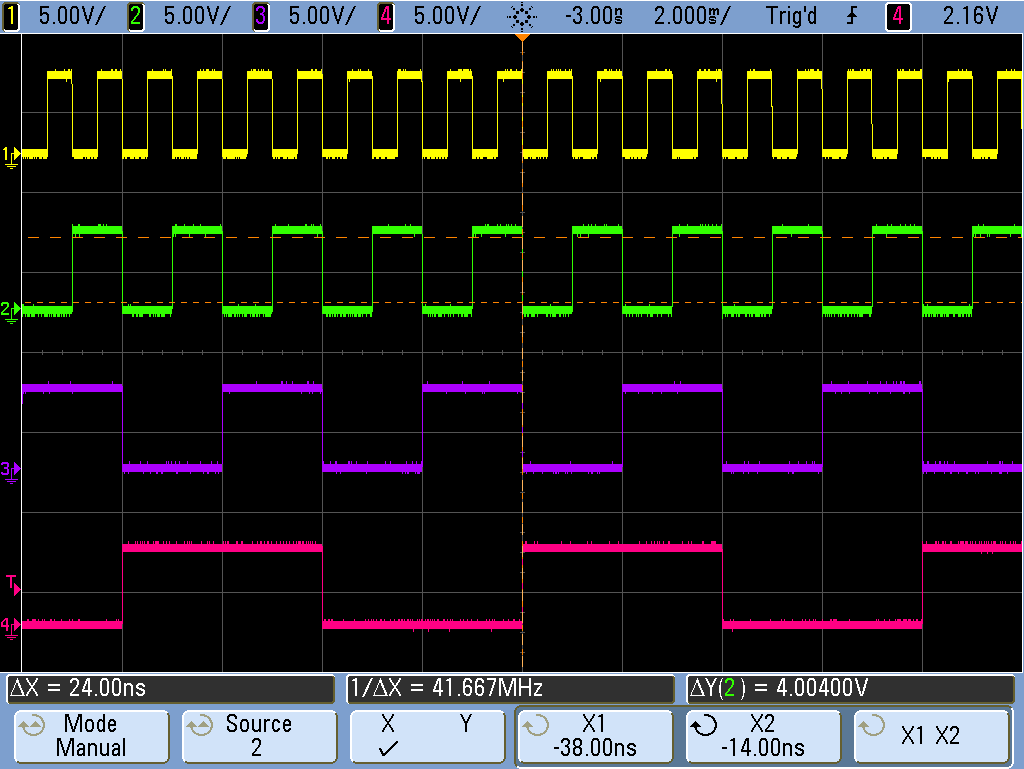
\includegraphics[scale=0.2]{ejercicio7/imagenes/sync25.png}
  	\end{center}
  \caption{Comportamiento a bajas frec}
  \label{7_fig8}
  \end{minipage}
  \begin{minipage}[b]{0.4\textwidth}
  	\begin{center}
  		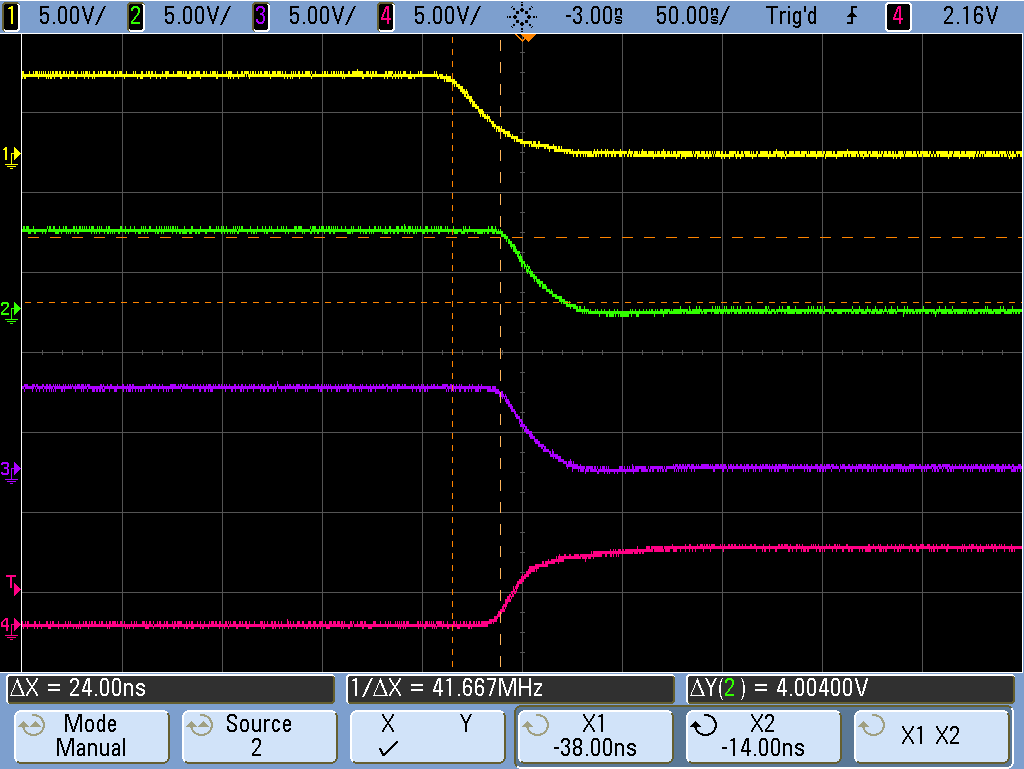
\includegraphics[scale=0.2]{ejercicio7/imagenes/sync24.png}
  	\end{center}
  \caption{Medición del tiempo de propagación}
  \label{7_fig9}
  \end{minipage}
\end{center}
\end{figure}
